%\documentclass[handout]{beamer}
\documentclass{beamer}

\usepackage{beamerthemesplit}
\usepackage{shadowtext}
\usepackage{color}
\usepackage{xcolor}
\usepackage[utf8]{inputenc}

 \usetheme[]{Madrid}
%\usetheme[]{Copenhagen}
%\usetheme{Warsaw}

% El que uso habitualmente:
%\usetheme[height=0.7cm]{Rochester}

% A dark look
%\usecolortheme{beetle}
% A light look:
 \usecolortheme{dolphin}
 
\setbeamertemplate{footline}
{
  \leavevmode%
  \hbox{%
  \begin{beamercolorbox}[wd=.5\paperwidth,ht=2.25ex,dp=1ex,center]{author in head/foot}%
    \usebeamerfont{author in head/foot}\insertshortauthor
  \end{beamercolorbox}%
  \begin{beamercolorbox}[wd=.5\paperwidth,ht=2.25ex,dp=1ex,center]{title in head/foot}%
    \usebeamerfont{title in head/foot}\insertshorttitle\hspace*{3em}
    \insertframenumber{} / \inserttotalframenumber\hspace*{1ex}
  \end{beamercolorbox}}%
  \vskip0pt%
}
\makeatletter

\setbeamertemplate{navigation symbols}{} 

%\usepackage{wrapfig}
\setbeamercovered{transparent}

\usepackage{geometry}
%\geometry{landscape}
\usepackage{multimedia}

\usepackage{bm}%bold matH

%\usepackage{shade}
\usepackage{fancybox}
 
\usepackage{amssymb}


% Defino clases de secciones en ESPAÑOL
\def\chaptername{Cap\'\i tulo}
\def\abstractname{Resumen}
\def\contentsname{Contenidos}
\def\bibname{Bibliograf\'\i a}
\def\appendixname{Ap\'endice}
\def\tablename{\textbf{Tabla}}
\def\figurename{\textbf{Figura}}
%\usepackage[dvips]{graphics,color,epsfig}
%\usepackage{pst-all}
%\usepackage{pstricks}
%\topmargin=-2cm  

% Defino formatos
\def\titulo#1{\frametitle{{\ \hfill {\bf #1}}}}
\def\figu#1{\shadowbox{#1}}

%EStilo
%\input{epsf.sty}

%Paquetes a utilizar

%\usepackage{amssymb} % Math
%\usepackage{graphicx}
%\usepackage{float}
%%\usepackage{wrapfig}
%%\usepackage{deluxetable}

\pagenumbering{arabic}
%\usepackage[dvips]{graphics,color}
%\usepackage{natbib}
%\usepackage{amssymb} % Math
%\usepackage{amsmath} % Math
%%\usepackage{dsfont} % Math
%\usepackage{float}
%\usepackage{graphicx}
%%\usepackage{wrapfig}
%\usepackage{pst-all}
%%\usepackage{multirow} % Multi filas

%Separacion silabica:
%%\usepackage[T1]{babel} % silabas y hyphenation
%\hyphenation{e-vi-den-cia}
%\hyphenation{an-te-rio-res}

% Control de Márgenes

%-------------------- Comandos de los autores ----------------------------

% Nombres de Journals
\newcommand{\araa}{Annu. Rev. Astron. Astrophys.}
\newcommand{\solphys}{Solar Phys.}
\newcommand{\aapr}{Astron. Astrophys. Rev.}
\newcommand{\aaps}{Astron. Astrophys. Sup. Ser.}
\newcommand{\jastp}{Jour. Atmos. Solar-Terrestrial Phys.}
\newcommand{\pasj}{Pub. Astron. Soc. Japan}
\newcommand{\etal}{et al.\ }
\newcommand{\ha}{H$\alpha$ }
\newcommand{\aap}{Astron. \& Astrophys.}
\newcommand{\apjs}{Astrophys J. Sup.}
\newcommand{\jgr}{Journal of Geophys. Res.}
\newcommand{\grl}{Geophys. Res. Let.}
\newcommand{\pre}{Physical Rev. E}
\newcommand{\adv}{Adv. in Space Res.}
\newcommand{\SpaceS}{Space Science Reviews}
\newcommand{\planss}{Planet. Space Sci.}
\newcommand{\nat}{Nature}
\newcommand{\apj}{The Astrophysical Journal}
\newcommand{\apjS}{The Astrophysical Journal Supplement}
\newcommand{\apjl}{The Astrophysical Journal Letters}
\newcommand{\mnras}{MNRAS}
\newcommand{\pasp}{Publications of the Astronomical Society of the Pacific}
\newcommand{\apss}{Astrophys. Space Sci.}

% Formato
\def\salto{\vskip 0.3cm}
\def\mediosalto{\vskip 0.15cm}
\def\saltito{\vskip 0.1cm}


% Math:
\def\deg{$^\circ$}
\def\rsun{R$_{\odot}$}
\def\bB{\mathbf{B}}
\def\bE{\mathbf{E}}
\def\dpar#1#2{\frac{\partial#1}{\partial#2}}
%color:
\def\red#1{{\textcolor{red}{#1}}}
\def\azul#1{{\textcolor{blue}{#1}}}

\def\Figura#1{Figura \ref{#1}}
\def\Figuras#1#2{Figuras \ref{#1} a \ref{#2}}
\def\Figurasy#1#2{Figuras \ref{#1} y \ref{#2}}
\def\Tabla#1{Tabla \ref{#1}}
\def\Eq#1{Ecuaci\'on (\ref{#1})}
\def\Eqs#1#2{Ecuaciones (\ref{#1})-(\ref{#2})}
\def\Eqn#1{Ecuaci\'on (\ref{#1})}
\def\eqsy#1#2{Ecuaciones (\ref{#1}) y (\ref{#2})}

\def\exp{{\rm exp}}
\def\ln{{\rm ln}}
\def\sin#1{{\rm sen}(#1)}
\def\cos#1{{\rm cos}(#1)}
\def\sec{{\rm sec}}
\def\erg{{\rm erg}}
\def\cm{{\rm cm}}
\def\km{{\rm km}}
\def\sr{{\rm sr}}
\def\Hz{{\rm Hz}}
\def\GHz{{\rm GHz}}
\def\kev{{\rm kev}}
\def\sfu{{\rm SFU}}
\def\K{{\rm K}}
\def\MK{{\rm MK}}
\def\AU{{\rm UA}}
\def\UA{{\rm UA}}
\def\Log10{{\rm log_{10}}}
\def\G{{\rm G}}
\def\gsun{g_{\odot}}
\def\Rsun{R_{\odot}}
\def\Msun{ M_{\odot}}
\def\Ne{N_\mathrm{e}}
\def\NH{N_\mathrm{H}}
\def\NHe{N_\mathrm{He}}
\def\me{m_\mathrm{e}}
\def\mH{m_\mathrm{H}}
\def\mHe{m_\mathrm{He}}
\def\Tm{T_m}
\def\Tfit{T_{\rm fit}}
\def\Tefit{T_{e,{\rm fit}}}
\def\Te{T_{\rm e}}
\def\TH{T_{\rm H}}
\def\THe{T_{\rm He}}
\def\l{\lambda_{{\rm N}}}
\def\WT{W_{T}}
\def\aTm{\left<\Tm\right>}
\def\dT{\Delta T}
\def\emisin{\zeta_k^{\rm (syn)}}
\def\emitom{\zeta_k^{\rm(tom)}}

\def\fa{f_{\alpha} ({\bf x},{\bf w},t)}
\def\ffa{f_\alpha}
\def\xt{({\bf x},t)}
\def\vt{({\bf v},t)}
\def\xw{({\bf x},{\bf w})}
\def\xwt{({\bf x},{\bf w},t)}
\def\fa{f_\alpha}
\def\ww{{\bf w}}
\def\xx{{\bf x}}
\def\uu{{\bf u}}
\def\kk{{\bf k}}
\def\V{{\bf V}}
\def\ga{{\bf \Gamma}}

\def\lD{\lambda_D}
\def\ve{v_{Te}}
\def\we{\omega_e}
%\def\me{m_e}

\def\dgdv{ \frac{\partial g}{\partial v} }

\def\dndt{ \frac{\partial n}{\partial t} }
\def\drhodt{ \frac{\partial \rho}{\partial t} }

\def\dfdt{ {{\partial f} \over {\partial t}} }
\def\dfdx{ {{\partial f} \over {\partial \xx}} }
\def\dfdw{ {{\partial f} \over {\partial \ww}} }

\def\ddv{ {{\partial} \over {\partial v}} }
\def\ddt{ {{\partial} \over {\partial t}} }
\def\ddx{ {{\partial} \over {\partial \xx}} }
\def\ddw{ {{\partial} \over {\partial \ww}} }

\def\ep{\epsilon}
\def\al{\alpha}
\def\om{\omega}
\def\EF{{\bf E}}
\def\BF{{\bf B}}
\def\dl{\lambda_D}

\def\wp{\om_{pe}}
\def\P{\buildrel =\over P}

\def\intindef{\int_{0}^{\infty}}
%-----------Albert's-----------------
\def\rmax{$R_{\rm max}$}
\def\Nrad{N_r}
\def\Nlat{N_\theta}
\def\Nlon{N_\phi}
\def\bzeta{\boldsymbol{\zeta}}
\def\bI{{\boldsymbol{I}}}
\def\bW{{\bf W}}
\def\bp{{\boldsymbol{p}}}
\def\bR{{\bf R}}
\def\AFe{A_{\rm Fe}}
\def\br{{\bf r}}
\def\bl{{\boldsymbol{\lambda}}}
\def\Tab#1{Tabla \ref{#1}}
\def\Tmin{T_{\rm min}}
\def\Tmax{T_{\rm max}}
\def\intmm{\int_{\Tmin}^{\Tmax}}

%------------------------de albert

%---------- Author's commands---------------------------------

\def\bu{\textcolor{red}{\textbullet~}}
\def\tr{\bu}
\def\bbu{\textbullet~}
\def\btr{\textcolor{blue}{$\triangleright$~}}
\def\cmsq{cm$^2$}
\def\cmcu{cm$^3$}
\def\azul#1{\textcolor{blue}{#1}}
\def\rojo#1{\textcolor{red}{#1}}
\def\verde#1{\textcolor{green}{#1}}
\def\orange#1{\textcolor{orange}{#1}}
\colorlet{green}{green!60!gray}

\def\rsun{R$_{\rm SUN}$}
\def\bA{{\bf A}}
\def\ba{{\boldsymbol{a}}}
\def\bB{{\bf B}}
\def\bb{{\bf b}}
\def\bC{{\bf C}}
\newcommand{\dd}{\mathrm{d}}
\def\bD{{\bf D}}
\def\bd{{\bf d}}
\def\be{{\boldsymbol{e}}}
\def\bF{{\bf F}}
\def\bff{{\bf f}}
\def\bg{{\bf g}}
\def\bG{{\bf G}}
\def\bh{{\bf h}}
\def\bH{{\bf H}}
\def\bi{{\bf i}}
\def\bI{{\boldsymbol{I}}}
\def\bk{{\bf k}}
\def\bK{{\bf K}}
\def\bM{{\bf M}}
\def\bn{{\boldsymbol{n}}}
\def\bv{{\boldsymbol{v}}}
\def\boo{{\boldsymbol{o}}}
\def\bp{{\boldsymbol{p}}}
\def\bP{{\bf $P$}}
\def\bq{{\boldsymbol{q}}}
\def\bQ{{\bf Q}}
\def\br{{\boldsymbol{r}}}
\def\bR{{\bf R}}
\def\bs{{\bf s}}
\def\bS{{\bf S}}
\def\bn{{\bf n}}
\def\bt{{\bf t}}
\def\bT{{\bf T}}
\def\bU{{\bf U}}
\def\bW{{\bf W}}
\def\bx{{\bf x}}
\def\by{{\bf y}}
\def\bSigma{{\bf \Sigma}}
\def\bLambda{{\bf \Lambda}}
\def\blambda{{\bf \lambda}}
\def\bN{{\bf \mathcal{N}}}
\def\bchi{\boldsymbol{\chi}}
\def\bxi{\boldsymbol{\xi}}
\def\bzeta{\boldsymbol{ \zeta}}
\newcommand{\lbl}{\mbox{\boldmath $\hat{l}$}}
\newcommand{\lpl}{\mbox{\boldmath $\hat{p}$}}
\def\deg{$^\circ$}
\def\mdeg{^\circ}
\def\bbp{{\bf p}}

%\def\tr{\textcolor{blue}{$\blacktriangleright$~}}
\def\bu{\textcolor{blue}{\textbullet~}}
\def\tr{\bu}
\def\bbu{\textbullet~}

\def\cmsq{cm$^2$}
\def\cmcu{cm$^3$}

\def\negro#1{\textcolor{black}{#1}}
\def\blanco#1{\textcolor{white}{#1}}
\def\azul#1{\textcolor{blue}{#1}}
\def\rojo#1{\textcolor{red}{#1}}
\def\verde#1{\textcolor{green}{#1}}
\def\orange#1{\textcolor{orange}{#1}}

\def\bL{{\bf L}}
\def\bE{{\bf E}}

% Author's commands:
\newcommand{\DT}{\Delta T}
\newcommand{\Tsyn}{T_{\rm Syn}}
\newcommand{\Texp}{T_{\rm exp}}
\newcommand{\seg}{{\rm seg}}


%Simbolos
\def\izquierda{\azul{$\bf\leftarrowtail$}}
\def\derecha{\azul{$\bf\rightarrowtail$}}

%Diego:
\def\mrsun{{\rm R_\odot}}
\def\avgTe{\left<T_e\right>}
\def\bfa#1{\textcolor{blue}{\bf\tt #1}}
\def\bfr#1{\textcolor{red}{\bf\tt #1}}
\def\bfg#1{\textcolor{green}{\bf\tt #1}}
\def\med{{\rm Med}}
\def\mean{{\rm Mean}}

%Colores:
\definecolor{darkcandyapplered}{rgb}{0.64, 0.0, 0.0}
\definecolor{bluegray}{rgb}{0.4, 0.6, 0.8}
\definecolor{darkmidnightblue}{rgb}{0.0, 0.2, 0.4}
\definecolor{azure(colorwheel)}{rgb}{0.0, 0.5, 1.0}
\definecolor{blue(ryb)}{rgb}{0.01, 0.28, 1.0}

\def\rojo#1{\textcolor{darkcandyapplered}{\bf #1}}
\def\azul#1{\textcolor{darkmidnightblue}{\bf #1}}
\def\azul#1{\textcolor{blue(ryb)}{\bf #1}}

\def\verde#1{\textcolor{green}{#1}}
\def\orange#1{\textcolor{orange}{#1}}
\def\lazul#1{\textcolor{blue}{#1}}
\def\eazul#1{\textcolor{blue}{\emph{#1}}}

\def\verde#1{\textcolor{green}{\bf #1}}
\def\rosa#1{\textcolor{pink}{\bf #1}}
\def\orange#1{\textcolor{orange}{#1}}

\renewcommand{\deg}{$^\circ$}
\newcommand{\mAU}{\rm{AU}}
\newcommand{\mhr}{\rm{hr}}

% Definiciones refinadas, suplantan previas:
\def\Ne{N_{\textsf{e}}}
\def\Te{T_{\textsf{e}}}
\def\MK{\textsf{MK}}
\def\kK{\textsf{kK}}
\def\Rs{{R}_\odot}
\def\deg{^\circ}
\def\cm{\textsf{cm}}
\def\sec{\textsf{sec}}
\def\erg{\textsf{erg}}
\def\d{\textsf{d}}

 \def\sin{\textsf{sin}}
 \def\cos{\textsf{cos}}
 \def\Vthper{V_{\textsf{th}\perp}}
\def\Vthpar{V_{\textsf{th}\parallel}}
\def\THper{T_{\textsf{H}\perp}}
\def\THpar{T_{\textsf{H}\parallel}}
\def\NH{N_{\textsf{H}}}
\def\TH{T_{\textsf{H}}}
\def\Np{N_{\textsf{p}}}
\def\log10{{\textsf{log}}_{10}}
\def\DH{D_{\textsf{H}}}
\def\Np{N_{\textsf{p}}}
\def\RH{R_{\textsf{H}}}
 \def\dnu{\textsf{d}\nu}


\title[Tomography: UCoMP versus AIA versus KCOR]
{\bf Tomography: UCoMP versus AIA versus KCOR}
\author[Vasquez \& Nuevo]
       {
       {\bf 
       Alberto M. Vasquez \& Federico A. Nuevo}
       \vskip 0.25cm
       {\bf 
\tiny
Instituto de Astronomía y Física del Espacio (IAFE), Buenos Aires--Argentina\\
       }
       }
\institute[]
{
\begin{center}
\framebox{
\includegraphics[height=0.125\linewidth]{fig/logo_IAFE.eps}}
\vskip 3cm
{\bf March 2025}
\end{center}
}

\begin{document}

\frame{
\titulo{Tomography: UCoMP versus AIA versus KCOR}
{\tiny\sf
\begin{itemize}
\item \azul{Solar rotational tomography (SRT)} makes use of 1/2 solar rotation (14-day) long sequences of coronal images to determine the \azul{3D distribution of various physical quantities} of the corona, depending on the observed wavelength range.
\salto
\item Using \azul{WL pB} images (e.g. KCOR, C2, Metis), SRT allows determination of the \azul{3D $\Ne$}.
\salto
\item Using \azul{EUV} images with a given filter (e.g. AIA 171\,\AA), SRT allows determination of the \azul{3D band-emissivity}.\\ 
Based on the reconstructed band-emissivity for various filters independently (e.g. AIA 171, 193, and 211\,\AA),\\ 
a local-DEM analysis can be carried out at each location of the corona to determine the \azul{3D $\Ne$} and \azul{$\Te$}.\\ 
The combined procedure is known as DEM-Tomography, or \azul{DEMT}.
\salto
\item Using \azul{UCoMP} total-line (wavelength-integrated) images, SRT allows determination of the \azul{3D line emissivity}.
\saltito
\noindent
\hrulefill
\salto
\item For a specific period (September 2022), we carried out:
\saltito
a) \azul{UCoMP-SRT} with 1074 and 1079 nm images to determine their respective \azul{3D emissivity maps}.\\
\ \ \ \ The 1074:1079 emissivity-ratio can then be used to determine 3D $\Ne$.
\saltito
b) \azul{AIA-DEMT} (using filters 171, 193 and 211\,\AA) to determine the \azul{3D $\Ne$} and \azul{$\Te$},\\
\ \ \ \ in turn used with CHIANTI to compute \azul{3D synthetic emissivity maps} for the lines at 1074 and 1079 nm.
\saltito
c) \azul{KCOR-SRT} to determine the 3D distribution of $\Ne$.
\salto
\item These instruments allow reconstructions over a common range of heights $1.1-1.2\,\Rs$. We compare:
\saltito 
1) The tomographic UCoMP-SRT line emissivities against the synthetic prediction based on AIA-DEMT.
\saltito
2) {The 3D $\Ne$ derived from UCoMP-SRT, derived from AIA-DEMT, and derived from KCOR-SRT.}
\salto
\noindent\rojo{Fede: los resultados de las diapos 4 y 5 están copiados de la presentación que brindé en HAO durante nuestra visita pasada a UM. Entiendo que estos NO son los resultados más actuales, en particular que no tienen el ajuste de KCOR por pasar de mean-disk and disk-center Bsun. Cuando veas esto a la vuelta te pido actualices los gráficos con los correctos. Si querés podés subirlos vos mismo al repo, con igual nombre, y avisarme que haga pull.}
\end{itemize}
}}

\frame{
\titulo{3D Coronal Emissivity at 1074 nm}
{\footnotesize\sf
\begin{center}
Lat/Lon maps of UCoMP 3D \azul{Tomographic} 1074-Emissivity\\
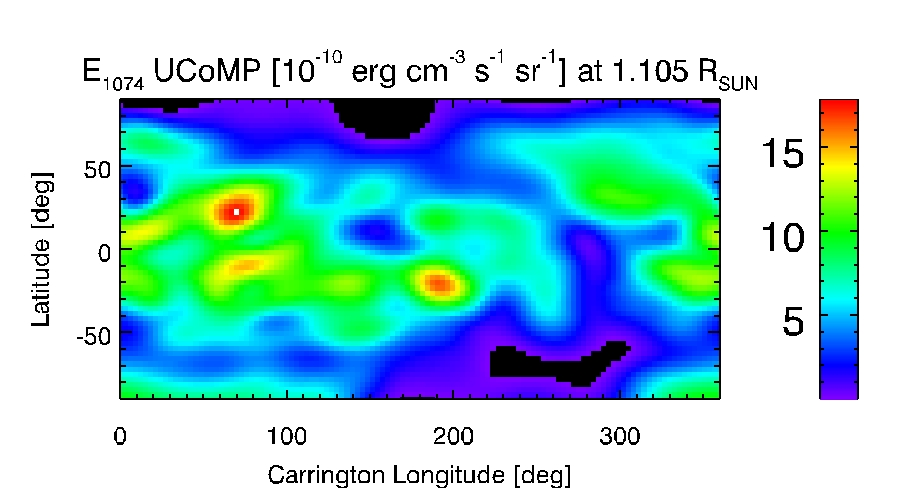
\includegraphics[width=0.32\textwidth,clip=]{fig/x_comp1074_1_105_Rsun.jpg}
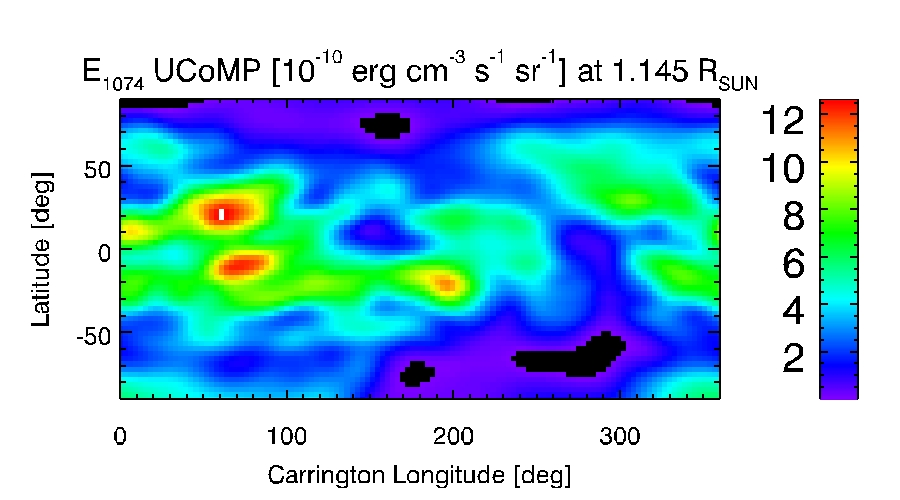
\includegraphics[width=0.32\textwidth,clip=]{fig/x_comp1074_1_145_Rsun.jpg}
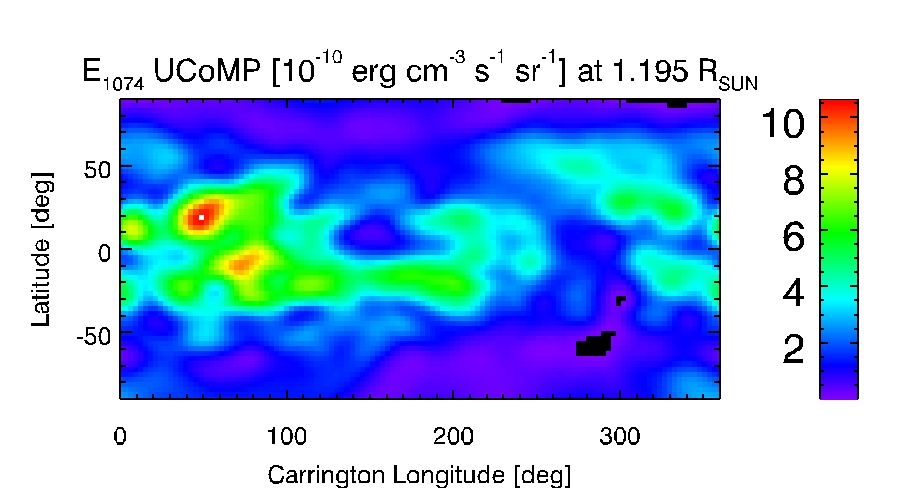
\includegraphics[width=0.32\textwidth,clip=]{fig/x_comp1074_1_195_Rsun.jpg}
\salto
Lat/Lon maps of AIA(171-193-211)-DEMT 3D \azul{Synthetic} 1074-Emissivity\\
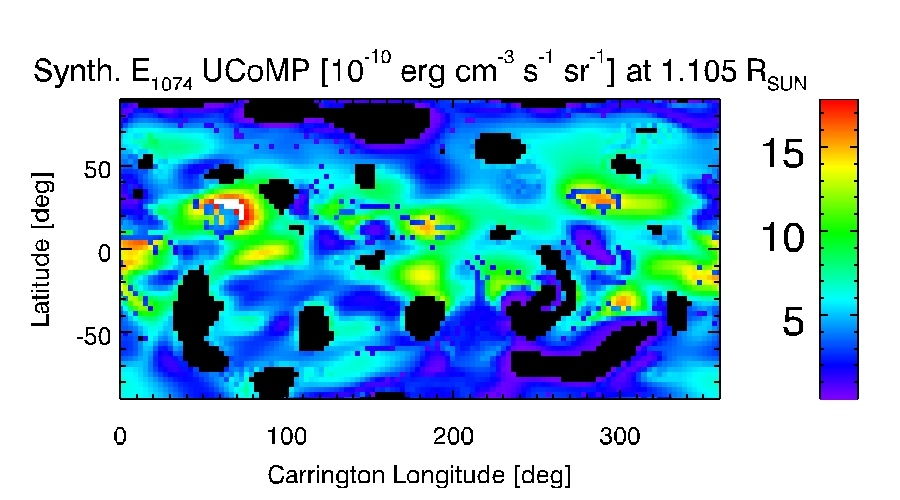
\includegraphics[width=0.32\textwidth,clip=]{fig/x_comp1074_synth_1_105_Rsun.jpg}
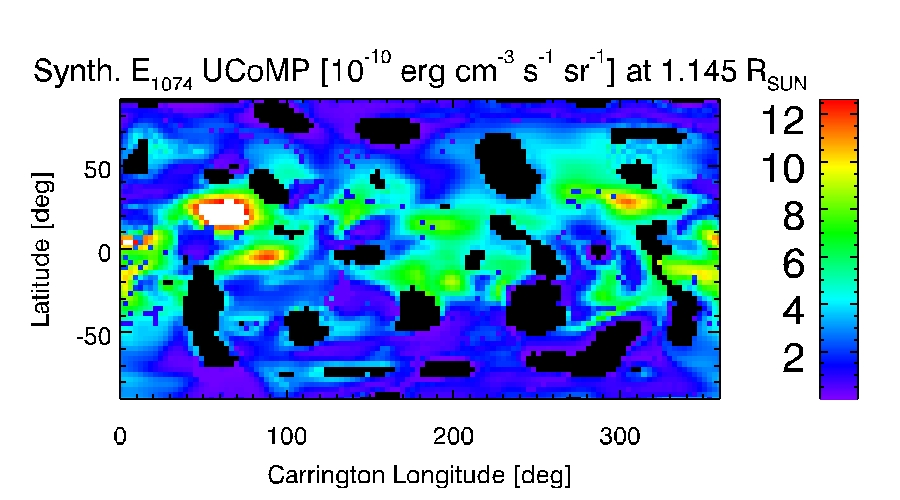
\includegraphics[width=0.32\textwidth,clip=]{fig/x_comp1074_synth_1_145_Rsun.jpg}
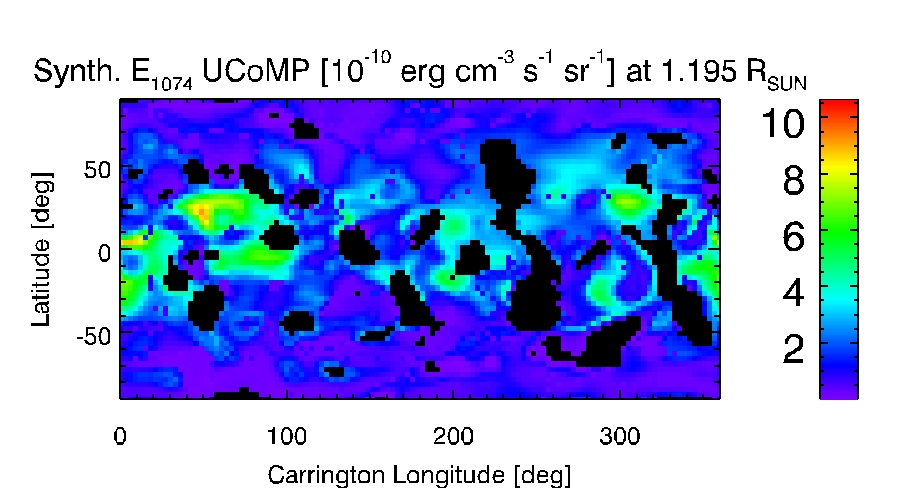
\includegraphics[width=0.32\textwidth,clip=]{fig/x_comp1074_synth_1_195_Rsun.jpg}
\salto
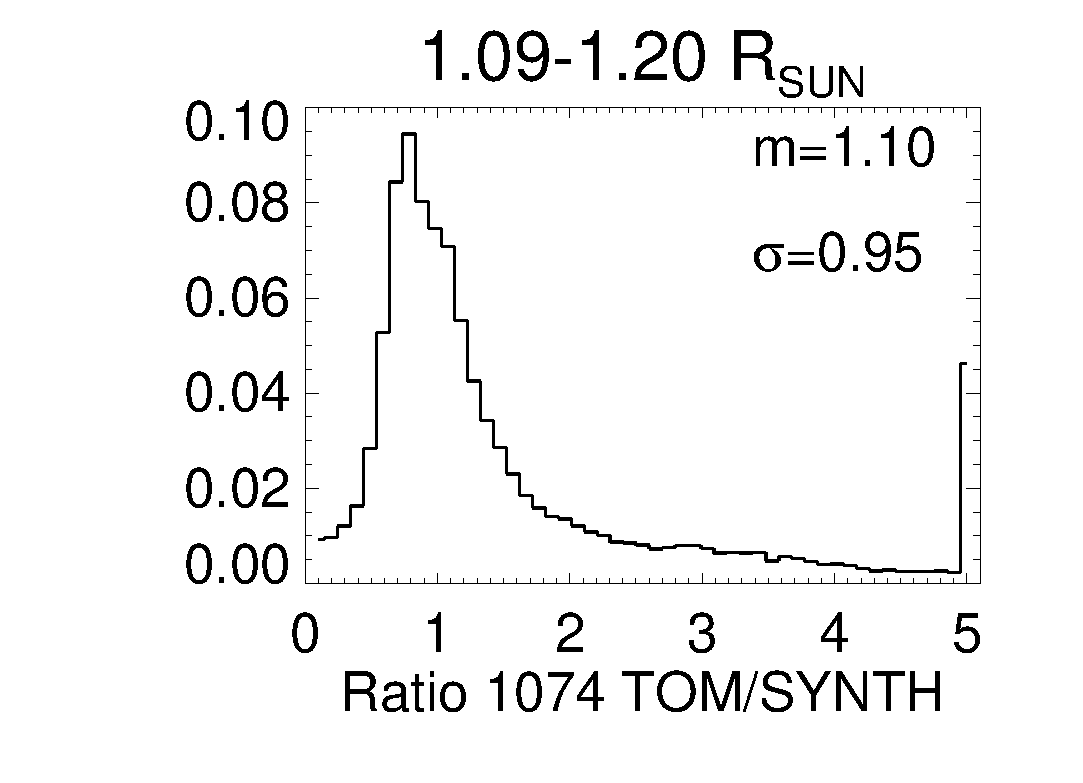
\includegraphics[height=0.2\textwidth,clip=]{fig/comparison_ucomp_Sept2022_tom_vs_synth_E1074_ratio_range1_090-1_200_Rsun.eps}
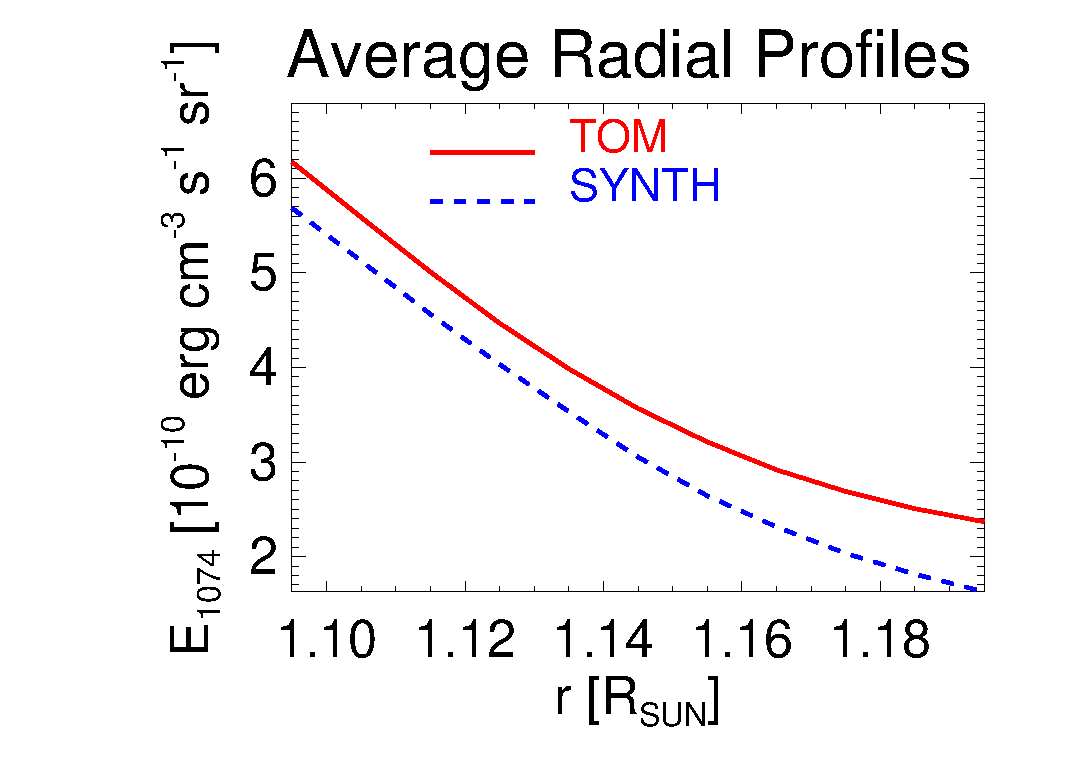
\includegraphics[height=0.2\textwidth,clip=]{fig/Average_Radial_Profiles_ucomp_Sept2022_tom_vs_synth_E1074.eps}
\end{center}
}
}

\frame{
\titulo{3D Coronal Emissivity at 1079 nm}
{\footnotesize\sf
\begin{center}
Lat/Lon maps of UCoMP 3D \azul{Tomographic} 1079-Emissivity\\
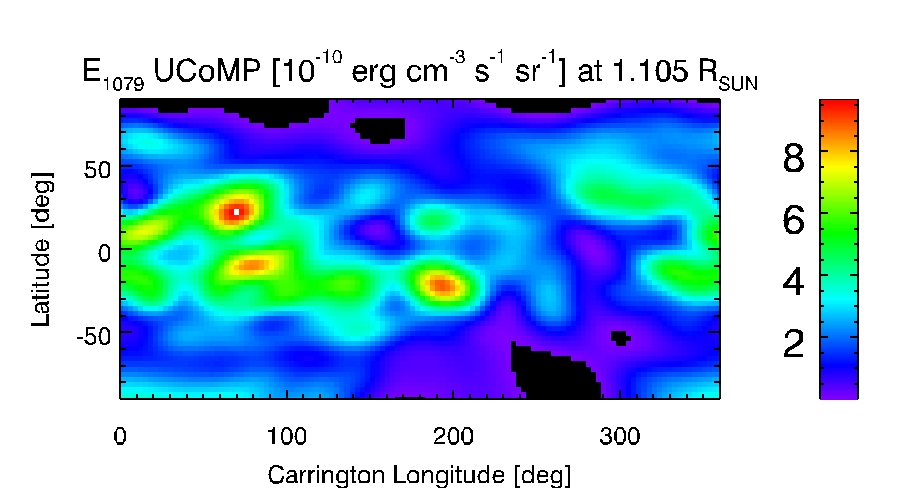
\includegraphics[width=0.32\textwidth,clip=]{fig/x_comp1079_1_105_Rsun.jpg}
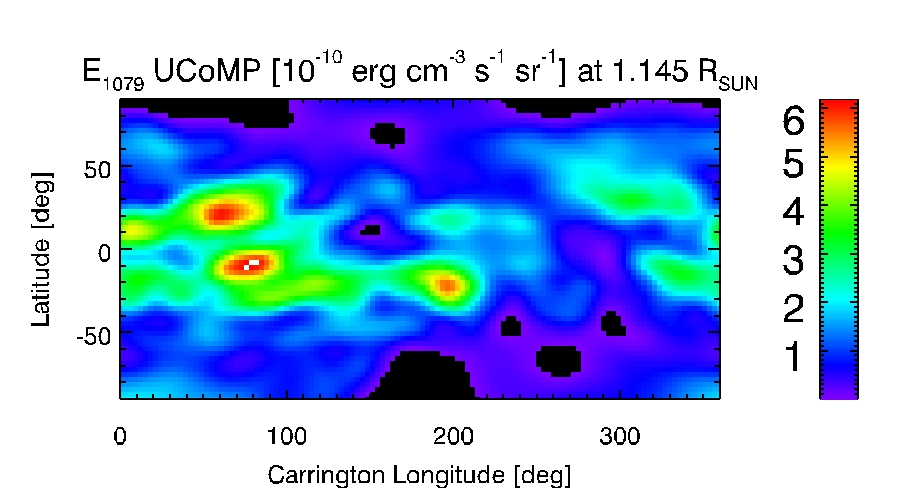
\includegraphics[width=0.32\textwidth,clip=]{fig/x_comp1079_1_145_Rsun.jpg}
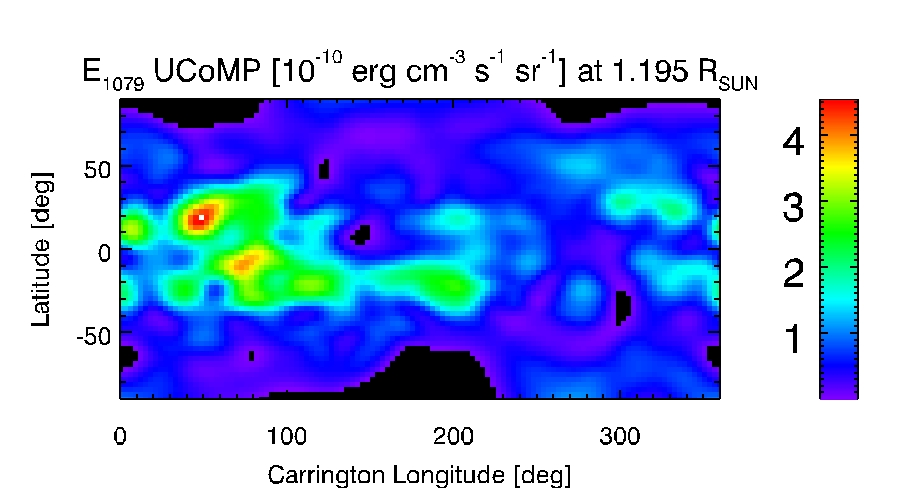
\includegraphics[width=0.32\textwidth,clip=]{fig/x_comp1079_1_195_Rsun.jpg}
\salto
Lat/Lon maps of AIA(171-193-211)-DEMT 3D \azul{Synthetic} 1079-Emissivity\\
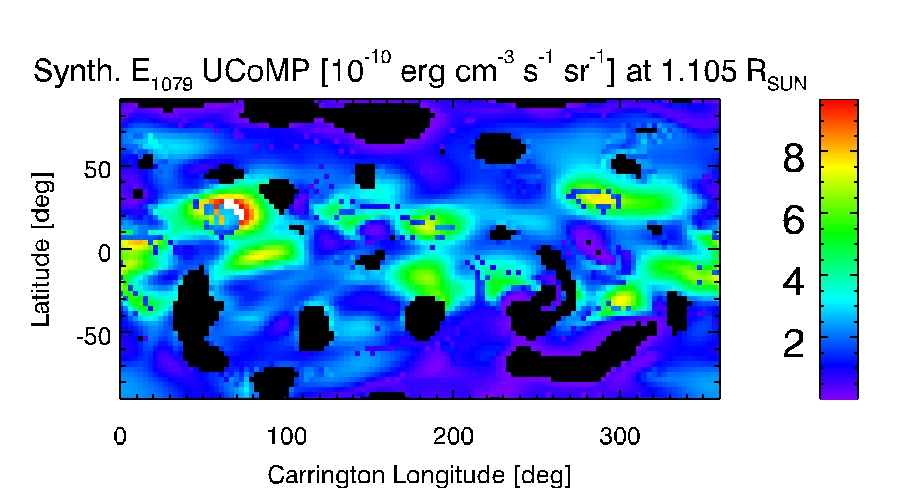
\includegraphics[width=0.32\textwidth,clip=]{fig/x_comp1079_synth_1_105_Rsun.jpg}
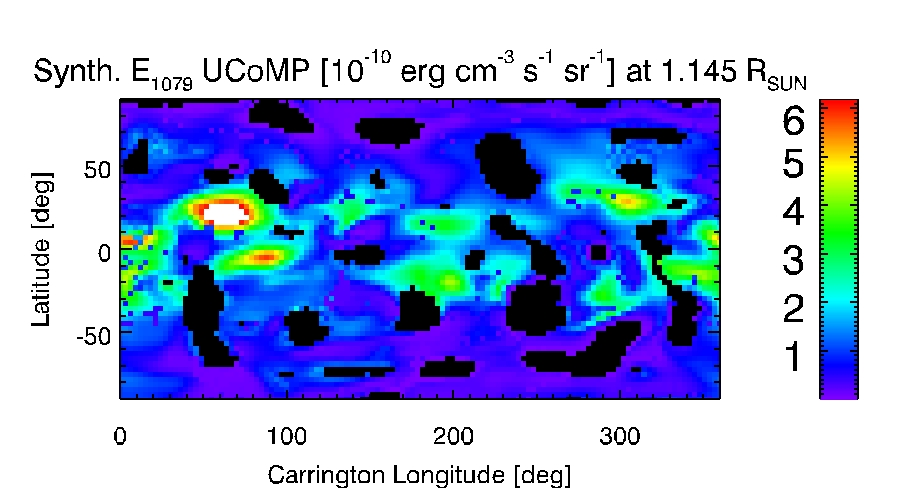
\includegraphics[width=0.32\textwidth,clip=]{fig/x_comp1079_synth_1_145_Rsun.jpg}
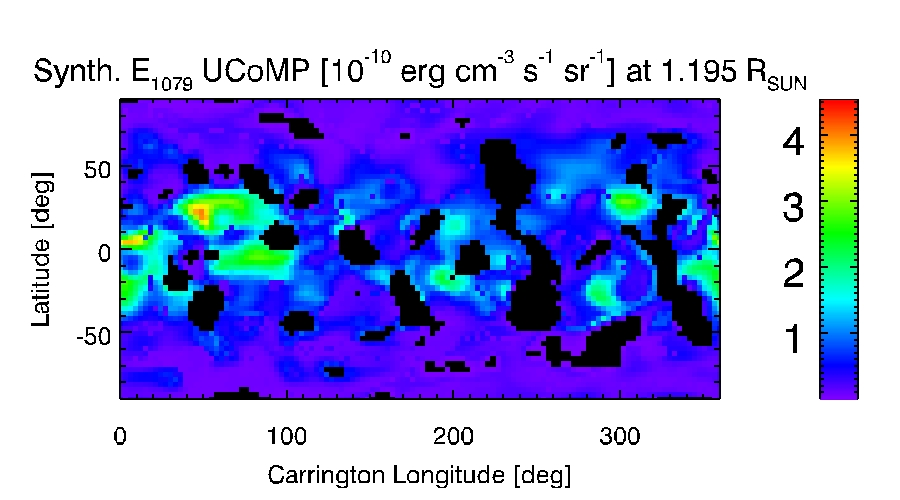
\includegraphics[width=0.32\textwidth,clip=]{fig/x_comp1079_synth_1_195_Rsun.jpg}
\salto
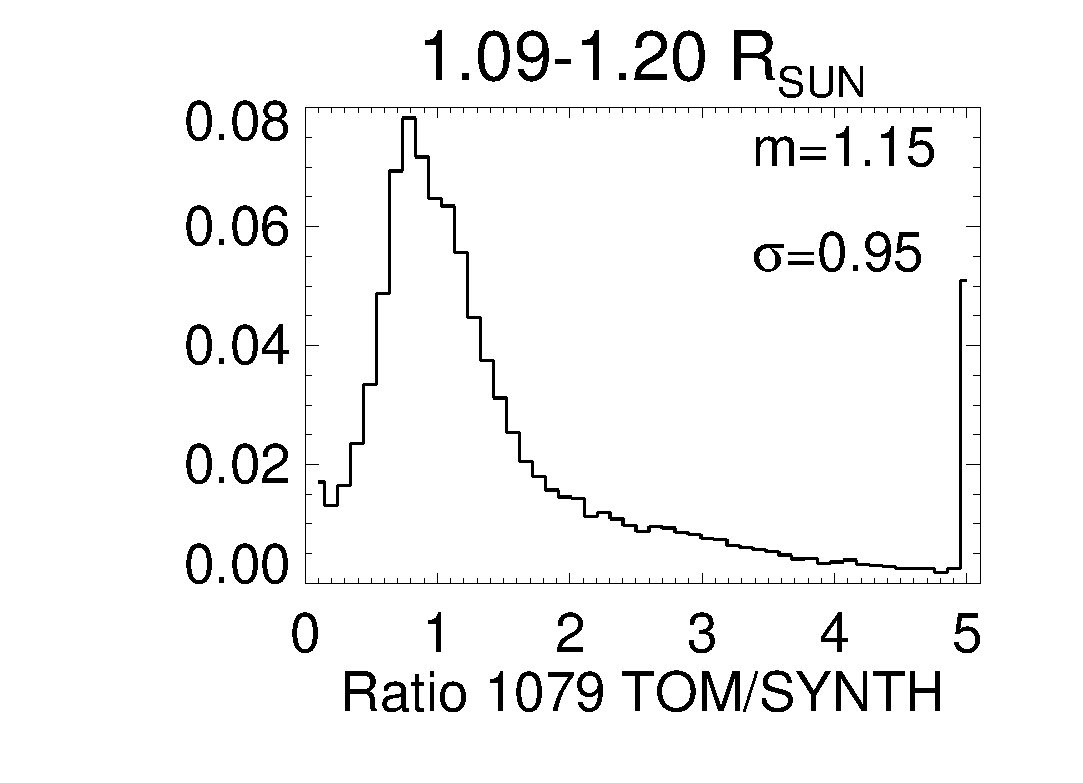
\includegraphics[height=0.2\textwidth,clip=]{fig/comparison_ucomp_Sept2022_tom_vs_synth_E1079_ratio_range1_090-1_200_Rsun.eps}
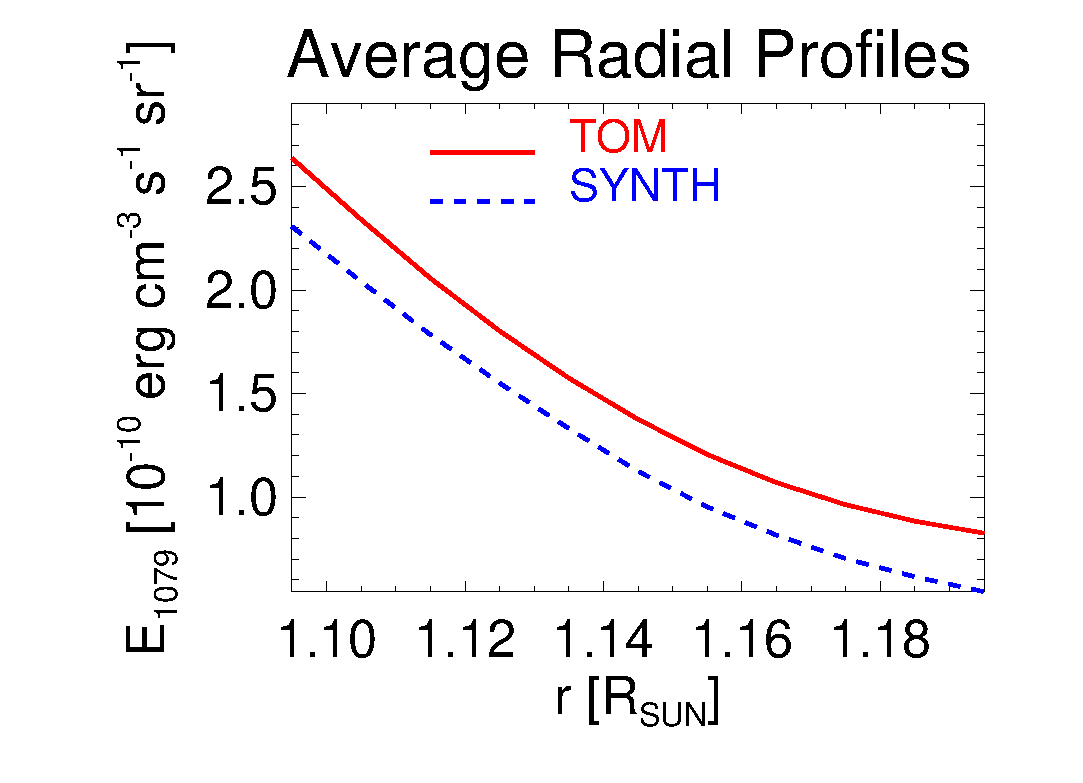
\includegraphics[height=0.2\textwidth,clip=]{fig/Average_Radial_Profiles_ucomp_Sept2022_tom_vs_synth_E1079.eps}
\end{center}
}
}


\frame{
\titulo{3D $\Ne$ with Three Diagnostics}
{\footnotesize\sf
\azul{
~~~~~~~UCoMP-SRT\hskip 2.2cm AIA-DEMT\hskip 2.3cm KCOR-SRT
}
\vspace{-0.1cm}
\begin{center}
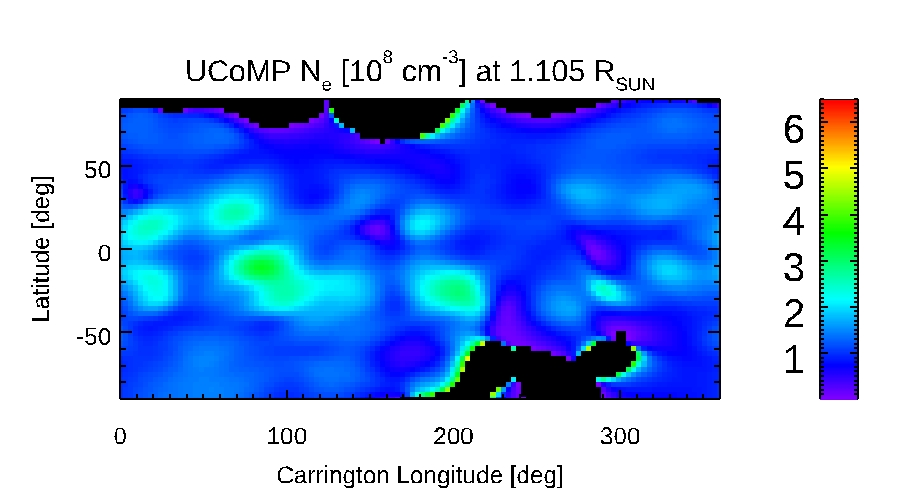
\includegraphics[width=0.32\textwidth,clip=]{fig/Ne_ucomp_1_105_Rsun.jpg}
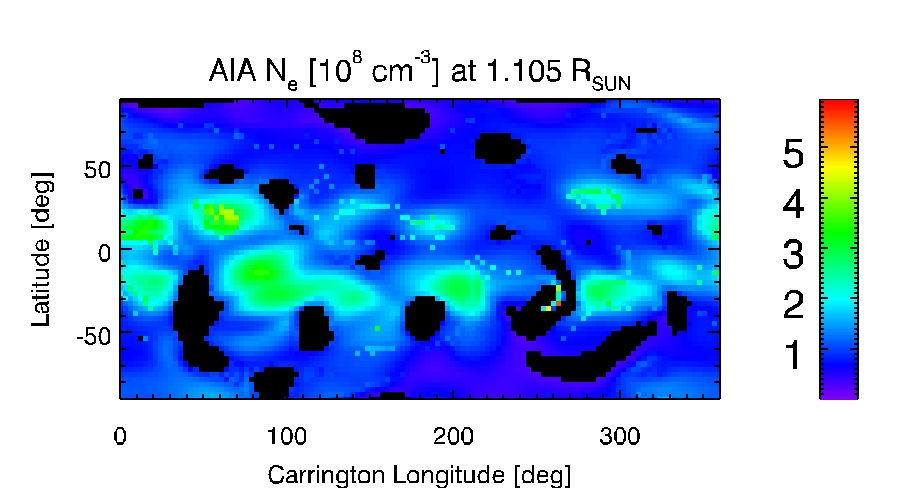
\includegraphics[width=0.32\textwidth,clip=]{fig/Ne_aia_1_105_Rsun.jpg}
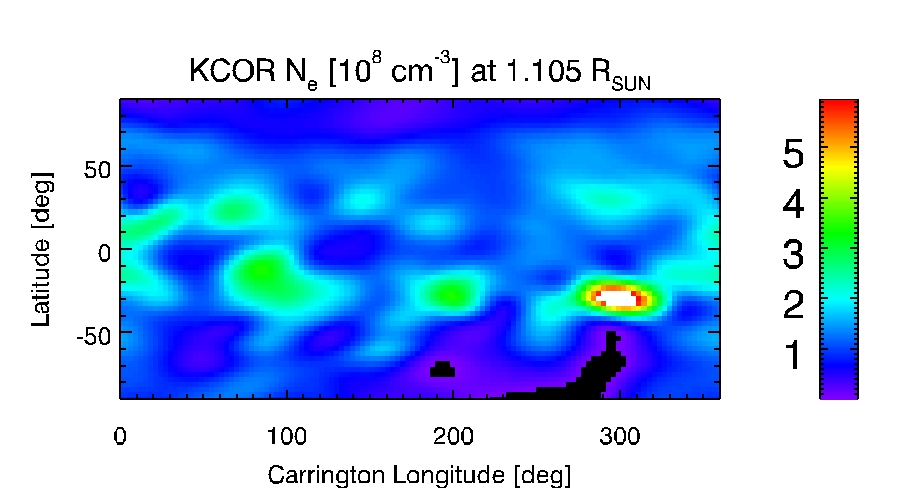
\includegraphics[width=0.32\textwidth,clip=]{fig/Ne_kcor_1_105_Rsun.jpg}
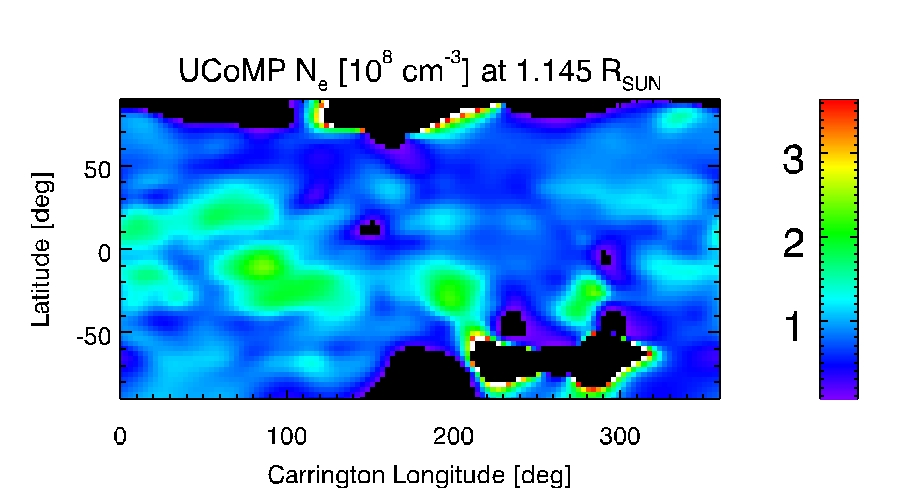
\includegraphics[width=0.32\textwidth,clip=]{fig/Ne_ucomp_1_145_Rsun.jpg}
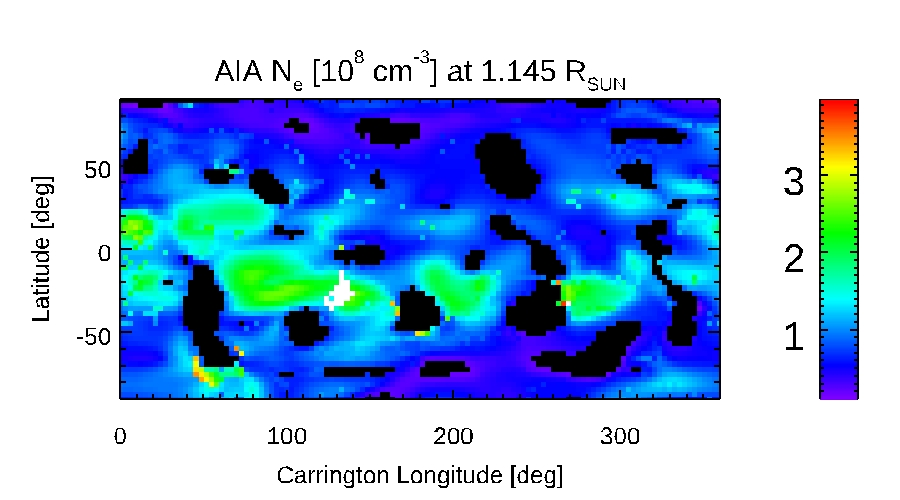
\includegraphics[width=0.32\textwidth,clip=]{fig/Ne_aia_1_145_Rsun.jpg}
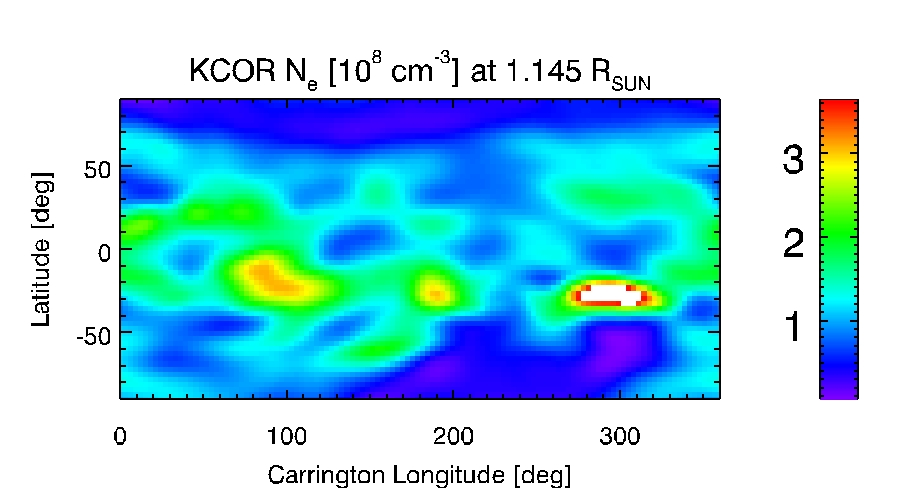
\includegraphics[width=0.32\textwidth,clip=]{fig/Ne_kcor_1_145_Rsun.jpg}
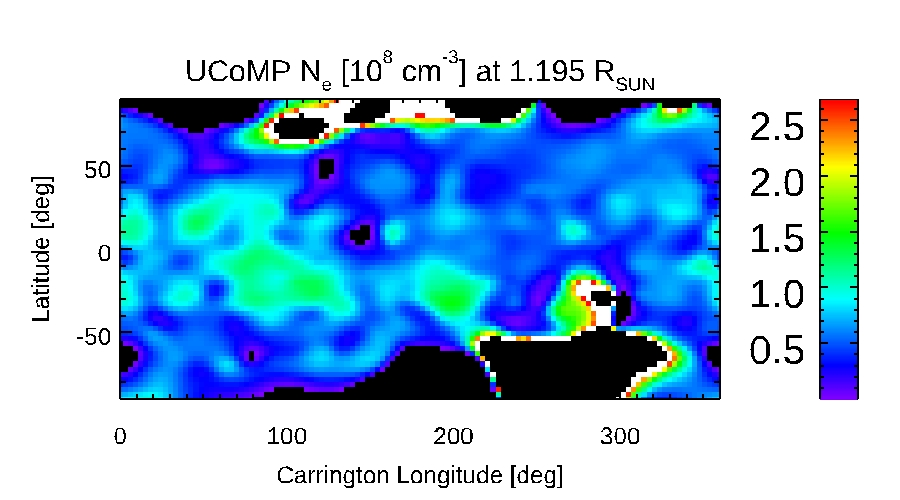
\includegraphics[width=0.32\textwidth,clip=]{fig/Ne_ucomp_1_195_Rsun.jpg}
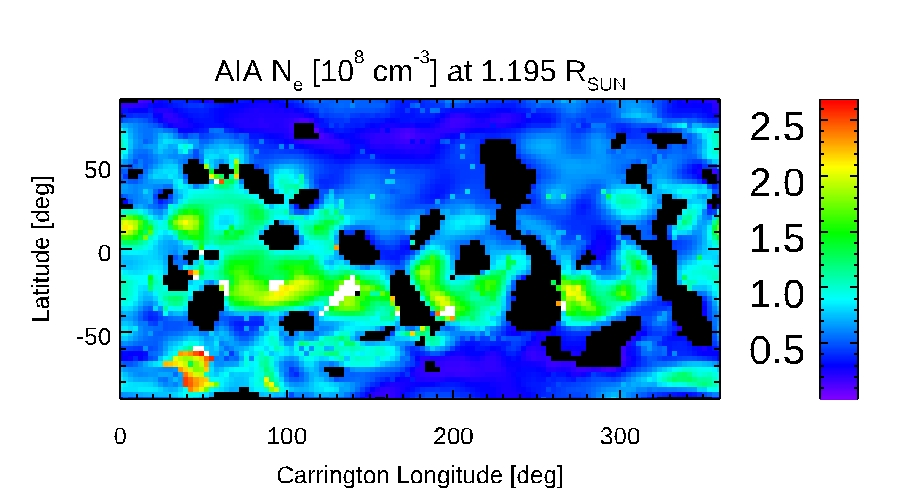
\includegraphics[width=0.32\textwidth,clip=]{fig/Ne_aia_1_195_Rsun.jpg}
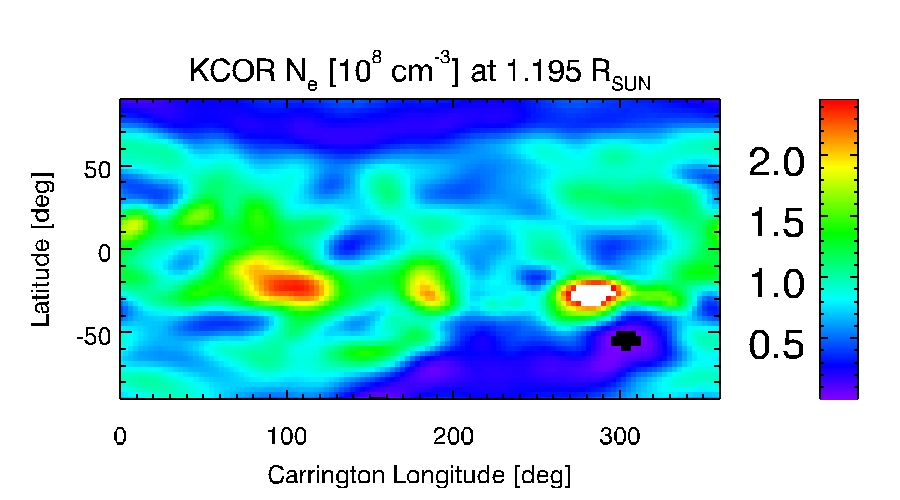
\includegraphics[width=0.32\textwidth,clip=]{fig/Ne_kcor_1_195_Rsun.jpg}
\end{center}
}
}

\frame{
\titulo{Comparison of Reconstructed $\Ne$}
{\footnotesize\sf
\vspace{+0.2cm}
\ \hskip 2.25cm {\bf UCoMP versus AIA \hskip 2.5cm UCoMP versus KCOR}
\begin{center}
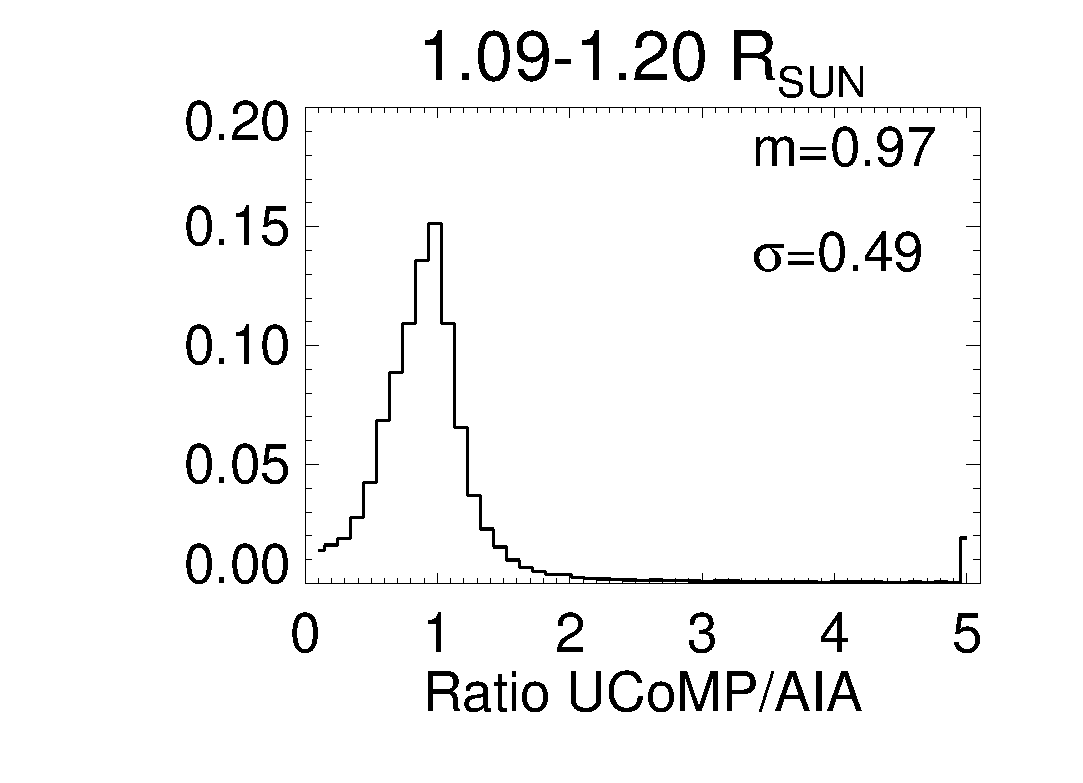
\includegraphics[width=0.45\textwidth,clip=]{fig/comparison_ucomp_vs_aia_ratio_range1_090-1_200_Rsun.eps}
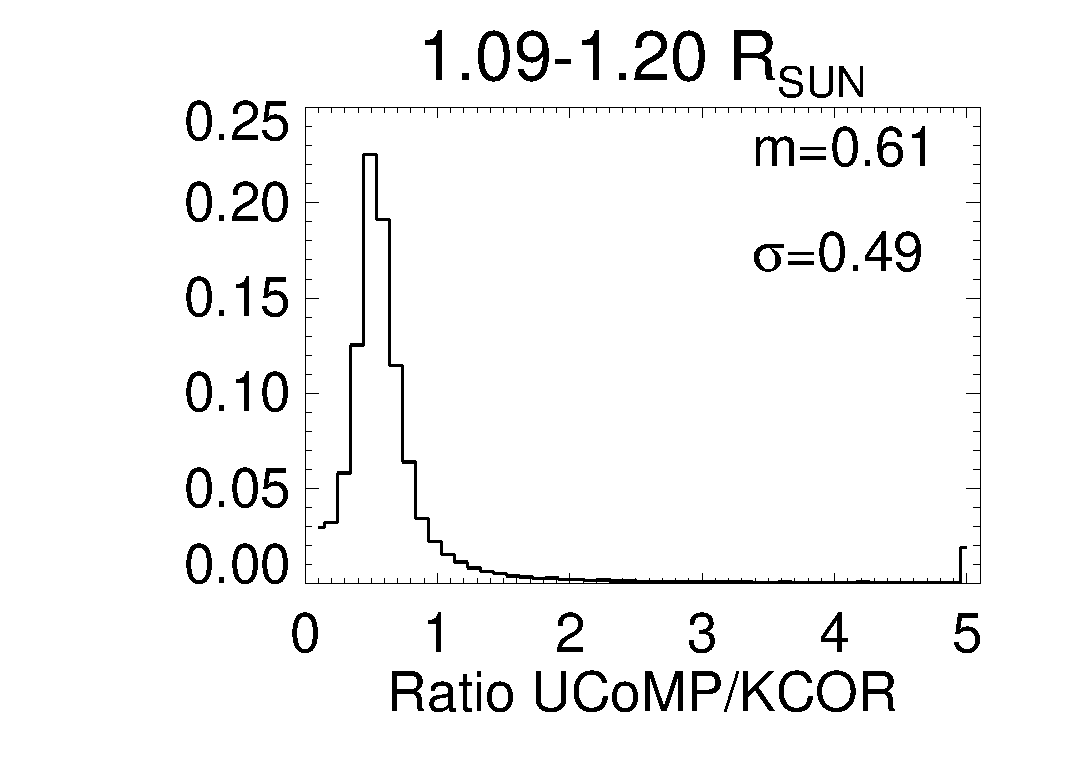
\includegraphics[width=0.45\textwidth,clip=]{fig/comparison_kcor_vs_ucomp_ratio_range1_090-1_200_Rsun.eps}
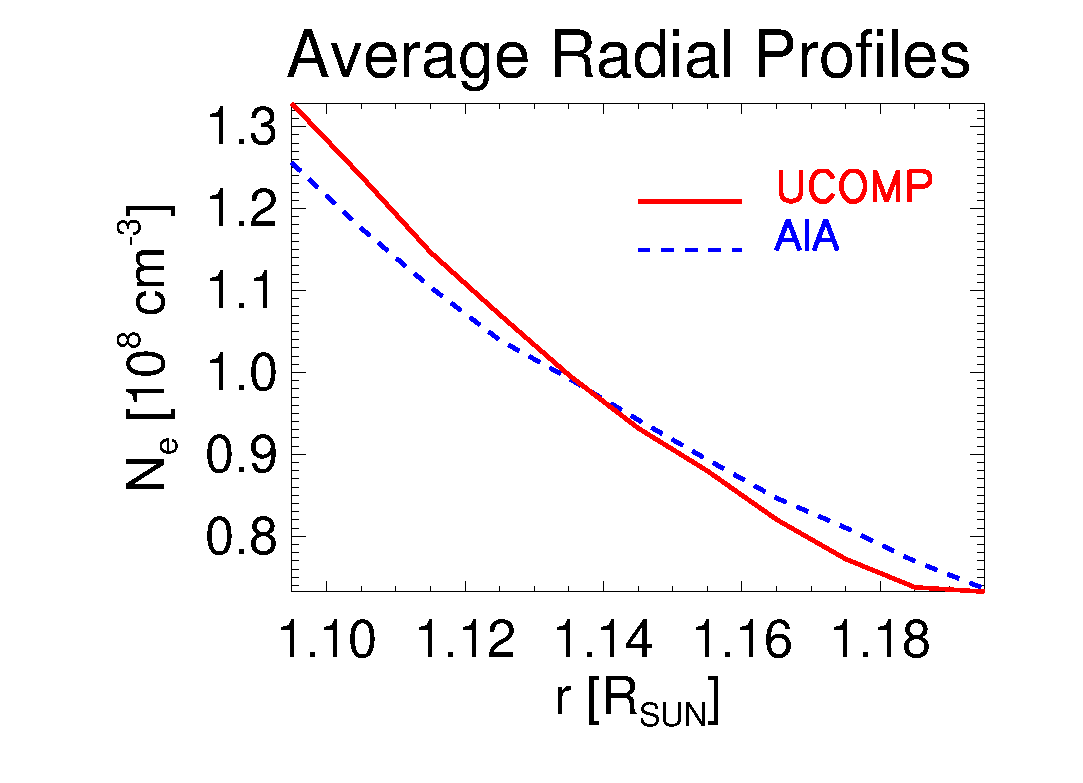
\includegraphics[width=0.45\textwidth,clip=]{fig/Average_Radial_Profiles_ucomp_vs_aia.eps}
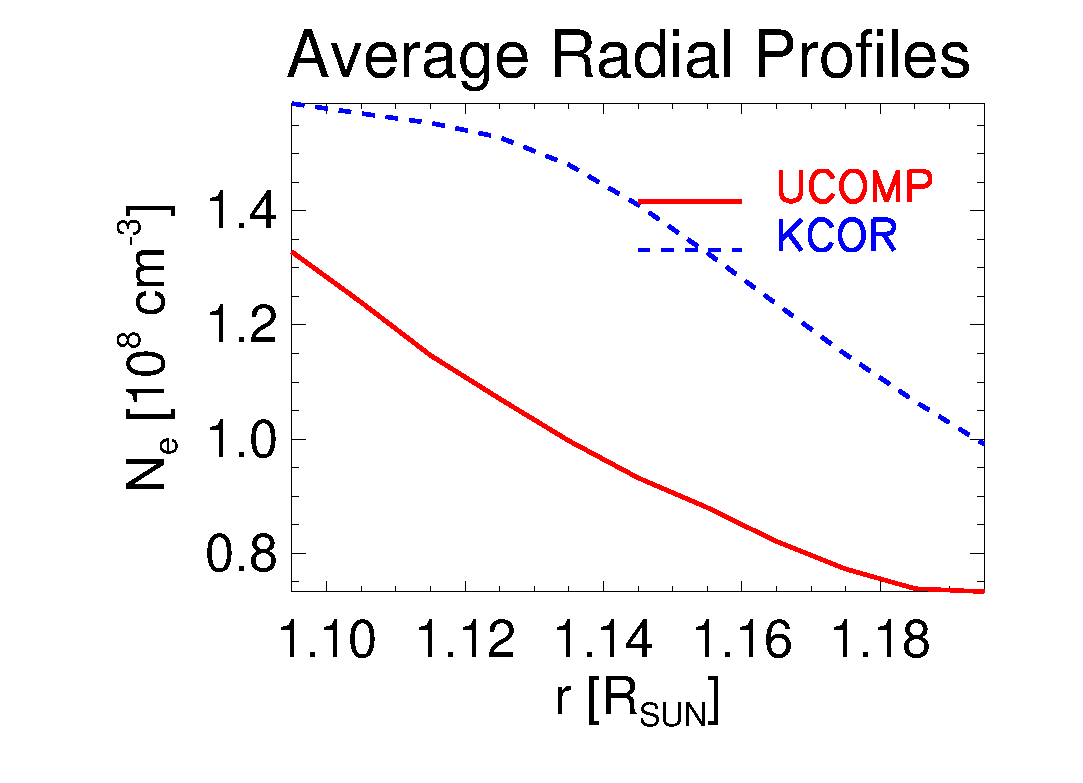
\includegraphics[width=0.45\textwidth,clip=]{fig/Average_Radial_Profiles_kcor_vs_ucomp.eps}
\end{center}
}
}

\frame{
\titulo{A Few Comments}
{\footnotesize\sf
\noindent\rojo{Solo copié los comments de las diapos de la charla de CO. Juntémonos a discutir y ver de enriquecer y avanzar en esto. Un comentario general: en las comparaciones previas (histogramas y perfiles radiales promedio) se incluyen todas las latitudes? Si es así, miremos que pasa si limitamos al rango $\pm 60$\,deg, como para eliminar las zonas donde UCoMP tiene muy mala señal.}
\begin{itemize}
\item The UCoMP 1074:1079 emissivity ratio provides a direct diagnostic of $\Ne$ that can be compared to those of DEMT or KCOR-SRT. In addition, the comparison of the UCoMP 3D tomographic emissivities against the DEMT+CHIANTI synthtic maps provides an indirect consistency check for $\Te$ as well.
\salto
\item Emission lines to which UCoMP and AIA are sensitive are produced by $\rm Fe$ ions.
\salto
\item While the UCoMP-SRT $\Ne$ is independent of $\rm[Fe]$, AIA-SRT $\Ne \propto 1/ \sqrt{\rm [Fe]}$. Comparison of their reconstructed $N_e$ can in principle provide constraints on the 3D distribution of $\rm[Fe]$, as well as the coronal filling factor affecting emission lines.
\salto
\item The significantly larger SRT-KCOR $\Ne$ compared to SRT-AIA $\Ne$ has been consistently found for other periods (\azul{Lloveras et al. 2019}). Discrepancy can be due to calibration issues, coronal $[\rm Fe]$, and/or coronal filling factor.
\end{itemize}
}
}
\end{document}

